\documentclass[journal]{IEEEtran}
%\IEEEoverridecommandlockouts
% The preceding line is only needed to identify funding in the first footnote. If that is unneeded, please comment it out.

% listings package for code blocks
\usepackage{listings}
\usepackage{xcolor}
\usepackage{cite}
\usepackage{verbatim}
\usepackage{graphicx}
\usepackage{parskip}
\usepackage{amsmath}

\begin{document}

% overfull \hbox .. too wide 
\setlength{\emergencystretch}{12pt}
%\setlength{\parskip}{0pt} % 1ex plus 0.5ex minus 0.2ex}
\setlength{\parindent}{10pt}

\definecolor{codegreen}{rgb}{0,0.6,0}
\definecolor{codegray}{rgb}{0.5,0.5,0.5}
\definecolor{codepurple}{rgb}{0.58,0,0.82}
\definecolor{backcolour}{rgb}{0.95,0.95,0.92}

\lstdefinestyle{mystyle}{
    backgroundcolor=\color{backcolour},   
    commentstyle=\color{codegreen},
    keywordstyle=\color{magenta},
    numberstyle=\tiny\color{codegray},
    stringstyle=\color{codepurple},
    basicstyle=\ttfamily,
    breakatwhitespace=false,         
    breaklines=true,      
    postbreak=\mbox{\textcolor{red}{$\hookrightarrow$}\space},           
    captionpos=b,
}

\lstset{style=mystyle}

\title{Evaluating the Performance of KNN Clustering Classification}

\author{
\IEEEauthorblockN{Lillian Mueller}
\IEEEauthorblockA{lmuelle1@umd.edu}
\\
\IEEEauthorblockN{Regina Hong}
\IEEEauthorblockA{rhong@umd.edu}
}

\maketitle

\begin{abstract}
\label{log:abstract}
Given a dataset of Iris characteristics, this report explored the development of a similarity model to classify Iris species. A K-Nearest Neighbor model was used in this classification process, varying the number of nearest neighbors and distance metric used during implementation. After performing several iterations of k-fold cross validation compared to a Decision Tree model as well as a Logistic Regression model, it was observed that the Euclidean and Manhattan metrics of determining nearest neighbors resulted in a higher accuracy model. Also, the K-NN model (with 10 nearest neighbors) generally performed better than the Decision Tree model but not as well compared to the Logistic Regression model. Examining the validation results of the K-NN model on the Iris dataset contributes to learning the difference in use and performance between several supervised models.

\end{abstract}

\section{Introduction}
K-nearest neighbors (K-NN) is a type of classification model using similarity to determine the class of a new data point based on the data point(s) around it \cite{b1}. Where this new data point falls with respect to the comparison data is based on the measures, or the features of a dataset. K-NN usually uses Euclidean distance to calculate the nearest neighbors, but other methods may be used. This kind of model works best on small datasets that do not have a lot of noise. 

The focal dataset is the Iris dataset, supplied by the sci-kitlearn module. This dataset contains four feature measurements for each Iris flower: sepal length, sepal width, petal length, and petal width. Alongside these features, the classification of each Iris flower is given; the flower is classified as setosa, versicolor, or virginica. The K-nearest neighbors model was developed using the \lstinline{neighbors.KneighborsClassifier} class under the same module. The model was created with the intent of seeing how accurate it would be in classifying an Iris flower based on its feature measurements. In addition to the K-NN model, a logistic regression model and a decision tree model were also generated to compare the generative performance of the three models with respect to the same dataset. 

In this study, we use both K-nearest neighbors and k-fold cross validation. To reduce confusion between the variables, nearest neighbor values will be denoted by K and number of folds in cross validation will be denoted by k.

The Methodology section outlines the methodology used in creating the Python-based K-NN model and its performance as compared to a decision tree and logistic regression model. The Results section explores the results from the methods used, and the importance of this investigation is reviewed in the Discussion section.


\section{Methodology}
This investigation entails using scikitlearn’s \lstinline{KNeighbors} function from the \lstinline{neighbors} module to develop the k-nearest neighbors model. Several Python packages were utilized including \lstinline{sklearn}, \lstinline{matplotlib}, \lstinline{pandas}, and \lstinline{numpy}. Specifically from \lstinline{sklearn}, we use the following modules: \lstinline{linear_model}, \lstinline{preprocessing}, \lstinline{model_selection}, \lstinline{metrics}, \lstinline{pipeline}, \lstinline{inspection}, and \lstinline{tree}. 

The Iris dataset was loaded as an \lstinline{sklearn.utils.Bunch} object called \lstinline{iris_data} via the \lstinline{load_iris()} function. To make the data easier to read, it was transformed into the \lstinline{df_iris} dataframe, where the data parameter was set as the \lstinline{data} attribute of the dataset and the columns parameter as the \lstinline{feature_names} attribute. A new column called “class” was added to this dataframe which contains the \lstinline{target} variable of the Iris dataset; this is the class of the Iris plant – setosa, versicolor, or virginica. Since the \lstinline{target} attribute contains an array with values from 0-2, the \lstinline{replace} function was used to map these numerical values to their corresponding classifications: setosa for \(0\), versicolor for \(1\), and virginica for \(2\). 

After the Iris dataset was loaded in and processed, it was split into a train group and test group using the \lstinline{test_train_split} function, with 2/3 of the data as the train group and the remainder as the test group. 

We created two functions; the first function uses \lstinline{KNeighborsClassifier} to perform K-NN on the testing and training data. The parameters include: testing and training data, nearest neighbor value, whether the data is scaled, and which method is used for the nearest neighbor distance calculation. The second function is used to plot the results of the K-NN model iterations. A \lstinline{Pipeline} was used so that when the Iris dataset is scaled data, it can be graphed \cite{b2}. The two features selected for all the K-NN graphs were sepal length and sepal width. 

Two \lstinline{KNeighborsClassifier} parameters: \lstinline{metric} and \lstinline{ n_neighbors} were altered to determine which combination resulted in the best performing K-NN model. Keeping k=5, the \lstinline{metric} parameter was set to \lstinline{euclidean}, \lstinline{manhattan}, and \lstinline{cosine}. These distance calculations were performed on both unscaled and scaled data. Then, setting \lstinline{metric = euclidean}, the K-NN model was tested with nearest neighbor values of 3, 5, and 10. 

To compare the results of the K-NN model with other models, we created a decision tree model and a linear regression model using the same methods from our previous studies \cite{b3}, \cite{b4}. For the linear regression model, \lstinline{penalty=None}, for the decision tree, \lstinline{criterion = entropy}, and for K-NN, \lstinline{n_neighbors=10, metric=euclidean}. K-fold cross validation \cite{b5} was used with k=5 folds to compare the mean and standard deviation of accuracy values among the three models. Additionally, the k value was changed to k=6, 8, 10, 12, and 14 to observe how the three models performed during multiple iterations of cross validation. 

\section{Results}

The results of changing the \lstinline{metric} parameter are shown below. Both scaled and unscaled data were used, but only the results of scaled data are graphed. 

The training data accuracy, testing data accuracy, and r2 score for Euclidean, Manhattan, and cosine distance calculations are shown in Table~\ref{table:accur5scaled}, with scaled data and a consistent nearest neighbor value of 5. 

\begin{table}[h!]
\centering
\begin{tabular}{ c | c c c }
Metric & Train Data Accuracy & Test Data Accuracy & r2 Score \\
\hline
Euclidean & 0.98 & 0.96 & 0.935442 \\
Manhattan & 0.98 & 0.96 & 0.935442 \\
Cosine & 0.94 & 0.82 & 0.709490 \\
\end{tabular}
\caption{Accuracy and r2 Scores for Euclidean, Manhattan, and Cosine Distance with Scaled Data}
\label{table:accur5scaled}
\end{table}

Figures~\ref{fig:euclk5},~\ref{fig:mank5}, and~\ref{fig:cosk5} show the K-NN classification plots stemming from each of the different distance calculations. Using Euclidean and Manhattan distance resulted in similar if not identical accuracy scores. The boundaries between the three Iris species are similar. Meanwhile, using cosine distance resulted in a worse performing model by comparison. The boundaries between Iris versicolor and Iris virginica are rather erratic, resulting in streaks instead of smooth boundaries.

\begin{figure}[h!]
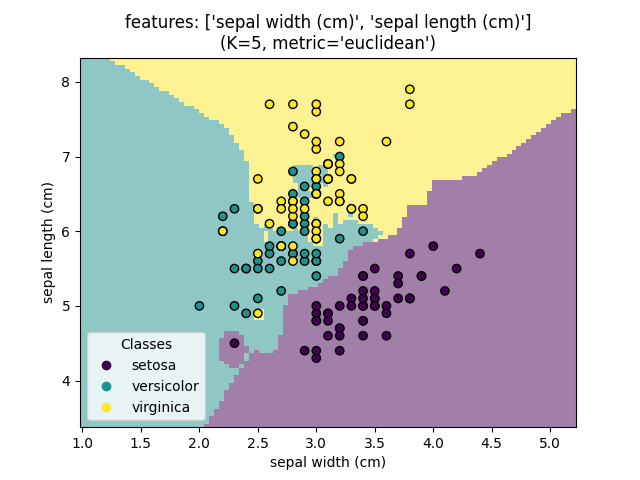
\includegraphics[scale=0.4]{euclidean_k5.png}
\centering
\caption{Euclidean Distance Metric with K=5}
\label{fig:euclk5}
\end{figure}

\begin{figure}[h!]
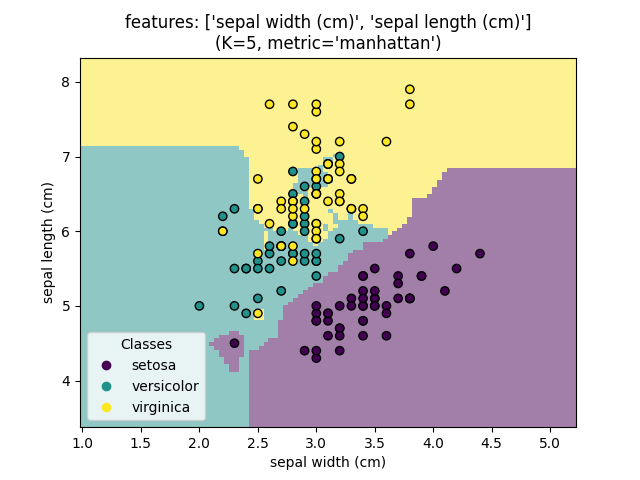
\includegraphics[scale=0.4]{manhattan_k5.png}
\centering
\caption{Manhattan Distance Metric with K=5}
\label{fig:mank5}
\end{figure}

\begin{figure}[h!]
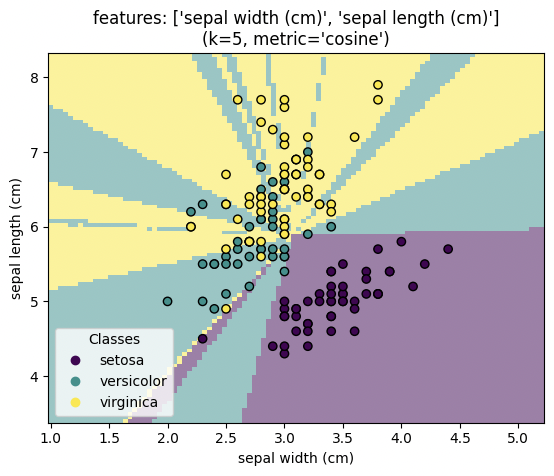
\includegraphics[scale=0.4]{cosine_k5.png}
\centering
\caption{Cosine Distance Metric with K=5}
\label{fig:cosk5}
\end{figure}

A look at using the same three distance measures, this time with unscaled data, is seen in Table~\ref{table:accur5unscaled}. Again, Euclidean distance and Manhattan distance both resulted in similar or identical accuracy and r2 scores. However, it looks like there is an improvement in cosine distance. 

\begin{table}[h!]
\centering
\begin{tabular}{ c | c c c }
Metric & Train Data Accuracy & Test Data Accuracy & r2 Score \\
\hline
Euclidean & 0.97 & 0.98 & 0.967721 \\
Manhattan & 0.97 & 0.98 & 0.967721 \\
Cosine & 0.98 & 0.96 & 0.935442 \\
\end{tabular}
\caption{Accuracy and r2 Scores for Euclidean, Manhattan, and Cosine Distance with Unscaled Data}
\label{table:accur5unscaled}
\end{table}

\newpage 

With the \lstinline{metric} parameter set to Euclidean distance, Table ~\ref{table:accurkscaled} shows the train and test data accuracies as well as the r2 score for different nearest neighbors values: K=3, 5, and 10. Figures~\ref{fig:euclk3} and~\ref{fig:euclk10} show the K-NN plots for K=3 and K=10 (refer to Figure~\ref{fig:euclk5} for K=5). A higher K-value resulted in smoother boundaries between the three Iris species.

\begin{table}[h!]
\centering
\begin{tabular}{ c | c c c }
Metric & Train Data Accuracy & Test Data Accuracy & r2 Score \\
\hline
K=3 & 0.97 & 0.96 & 0.935442 \\
K=5 & 0.98 & 0.96 & 0.935442 \\
K=10 & 0.96 & 0.96 & 0.935442 \\
\end{tabular}
\caption{Accuracy and r2 Scores for K=3, 5, 10 with Scaled Data}
\label{table:accurkscaled}
\end{table}


\begin{figure}[h!]

\includegraphics[scale=0.4]{euclidean_k3.png}
\centering
\caption{Euclidean Distance Metric with K=3}
\label{fig:euclk3}
\end{figure}

\begin{figure}[h!]
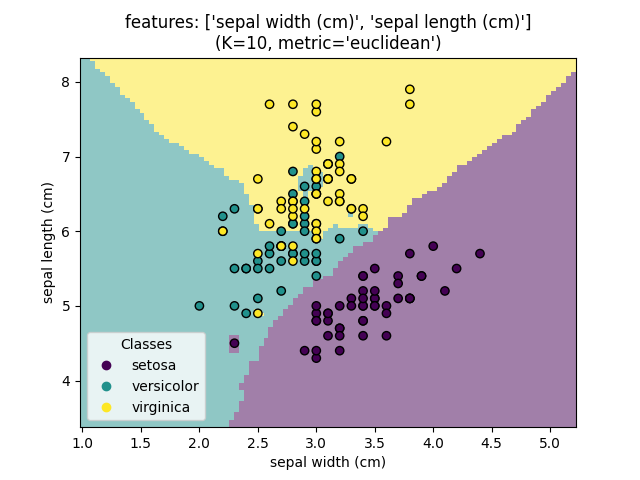
\includegraphics[scale=0.4]{euclidean_k10.png}
\centering
\caption{Euclidean Distance Metric with K=10}
\label{fig:euclk10}
\end{figure}

A generalized performance comparison of the K-NN model (using Euclidean distance and 10 nearest neighbors) with the decision tree and logistic regression models is shown below in Table~\ref{table:stats3models}. The number of folds for cross validation was set to k=5. It should be noted that the data was not scaled. The K-NN model resulted in highest accuracy.  

\begin{table}[h!]
\centering
\begin{tabular}{ c | c c c }
Statistic & Logistic Regression & Decision Tree & K-NN \\
\hline
Mean & 0.973333 & 0.96 & 0.98 \\
Standard Deviation & 0.036515 & 0.036515 & 0.029814 \\
\end{tabular}
\caption{Accuracy Statistics for Logistic Regression, Decision Tree, and K-NN, k=5 folds}
\label{table:stats3models}
\end{table}


Altering the number of folds in k-fold cross validation, the results for k=6, 8, 10, 12, and 14 are shown in Table~\ref{table:MultiFoldCV}.

\begin{table}[h!]
\centering
\begin{tabular}{ c | c c c }
Statistic & Logistic Regression & Decision Tree & K-NN \\
\hline
Mean (k=6) & 0.973333 & 0.96 & 0.966667 \\
Standard Deviation (k=6)  & 0.03266 & 0.035777 & 0.046762 \\
Mean (k=8) & 0.980263 & 0.953582 & 0.966740 \\
Standard Deviation (k=8)  & 0.039159 & 0.043997 & 0.039383 \\
Mean (k=10) & 0.98 & 0.953333 & 0.966667 \\
Standard Deviation (k=10)  & 0.044997 & 0.044997 & 0.04714 \\
Mean (k=12) & 0.966346 & 0.946581 & 0.965812 \\
Standard Deviation (k=12)  & 0.081228 & 0.062469 & 0.055233 \\
Mean (k=14) & 0.980519 & 0.940909 & 0.966883 \\
Standard Deviation (k=14)  & 0.03871 & 0.058019 & 0.046163 \\
\end{tabular}
\caption{Cross Validation Statistics for Logistic Regression, Decision Tree, and K-Nearest Neighbors Models (number of folds=6, 8, 10, 12, and 14)}
\label{table:MultiFoldCV}
\end{table}


\section{Discussion}
Through this study, we were able to confirm that a higher K or nearest neighbor value would result in smoother boundaries between the three Iris classes.  Among the decision tree, logistic regression, and K-nearest neighbor models, K-NN had the highest accuracy and smallest standard deviation values when only 5 folds were used. Seeing that nearly all the Iris setosa data points (\(\frac{1}{3}\) of the whole dataset) are apparently closely grouped together, it makes sense that a model that relies on distance as one of its parameters would result in high accuracy. It is interesting to note that beyond k=5 folds, the logistic regression model outperformed both the decision tree and K-NN models; the mean accuracy of the logistic regression model was higher than the other two models at k=6, 8, 10, 12, and 14 folds.

When the data was scaled, using Euclidean and Manhattan distance calculations resulted in higher accuracies than using the cosine calculation. The increase in accuracy using the cosine distance calculation when the data was unscaled could be attributed to the fact that it does not take into account the magnitudes of feature values. 

In the future, it would be beneficial to use other combinations of features (e.g., sepal length and petal length, sepal width and petal width, sepal length and petal width, etc.) to see which combination of features results in highest accuracy. Scaling the data may become much more important because the petal width values are much lower in magnitude than the other features, especially sepal length.

\newpage 

\begin{thebibliography}{00}
\bibitem{b1}
A. Kumar, “KNN Algorithm: What?When?Why?How?,” Medium. Accessed: Oct. 16, 2023. [Online]. Available: https://towardsdatascience.com/knn-algorithm-what-when-why-how-41405c16c36f
\bibitem{b2}
“Nearest Neighbors Classification,” scikit-learn. Accessed: Oct. 16, 2023. [Online]. Available: https://scikit-learn/stable/auto\_examples/neighbors/plot\_classification.html
\bibitem{b3}
L. Mueller and R. Hong, “Investigating Decision Trees,” Sep. 18, 2023.
\bibitem{b4}
L. Mueller and R. Hong, “Iris Classification Using Logistic Regression,” Sep. 25, 2023.
\bibitem{b5}
L. Mueller and R. Hong, “Using K-Fold Cross Validation on Decision Tree and Logistic Regression Models to Classify Iris Species,” Oct. 5, 2023.

\end{thebibliography}

\end{document}